The back-end readout card for the system under development, the Zynq UltraScale+ RFSoC ZCU216 Evaluation Card, was chosen taking into consideration the points described in \autoref{sec:selection}. In this section, the overall architecture and features of the card are presented. A possibility for evaluation of the card is also demonstrated. At last, a design for the read-out firmware is proposed. 

\section{Xilinx Zynq UltraScale+ RFSoC ZCU216 Evaluation Card}
Zynq UltraScale+ RFSoCs: Combine RF data converter subsystem and forward error correction with industry-leading
programmable logic and heterogeneous processing capability. Integrated RF-ADCs, RF-DACs, and soft decision FECs (SD-FEC)
provide the key subsystems for multiband, multi-mode cellular radios and cable infrastructure


With the data converters integrated directly into the FPGA using parallel interfaces, they don't require the
prohibitively high-pin-count external connections needed for discrete parallel interface converters, allowing more converter

\begin{itemize}[noitemsep]
	\item Sixteen 14-bit, 2.5GSPS RF-ADC
	\item Sixteen 14-bit, 10GSPS RF-DAC
	\item I/O expansion options – FPGA Mezzanine Card (FMC+) interfaces, RFMC 2.0 interfaces, and Pmod connections
\end{itemize}
\begin{figure}[tbh]
	\centering
	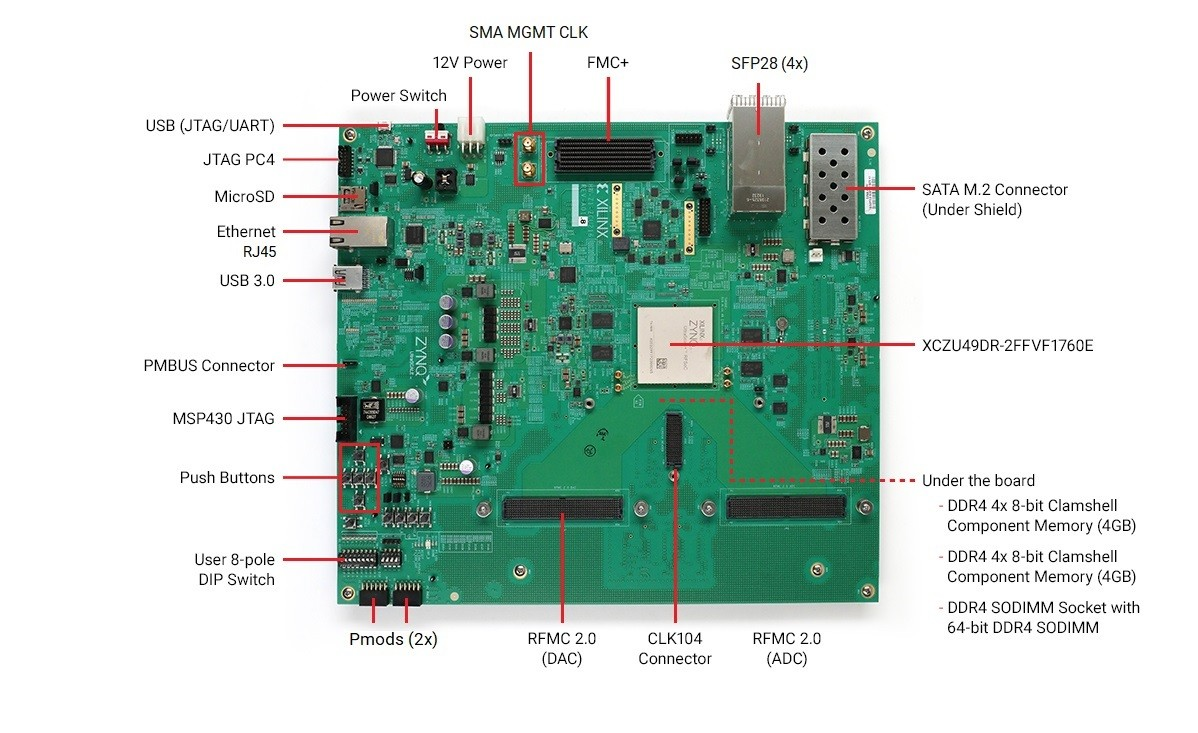
\includegraphics[width = \textwidth]{chap/04-work/img/zcu216}
	\caption{ZCU216 evaluation board}
	\label{fig:zcu216}
\end{figure}

\begin{figure}[tbh]
	\centering
	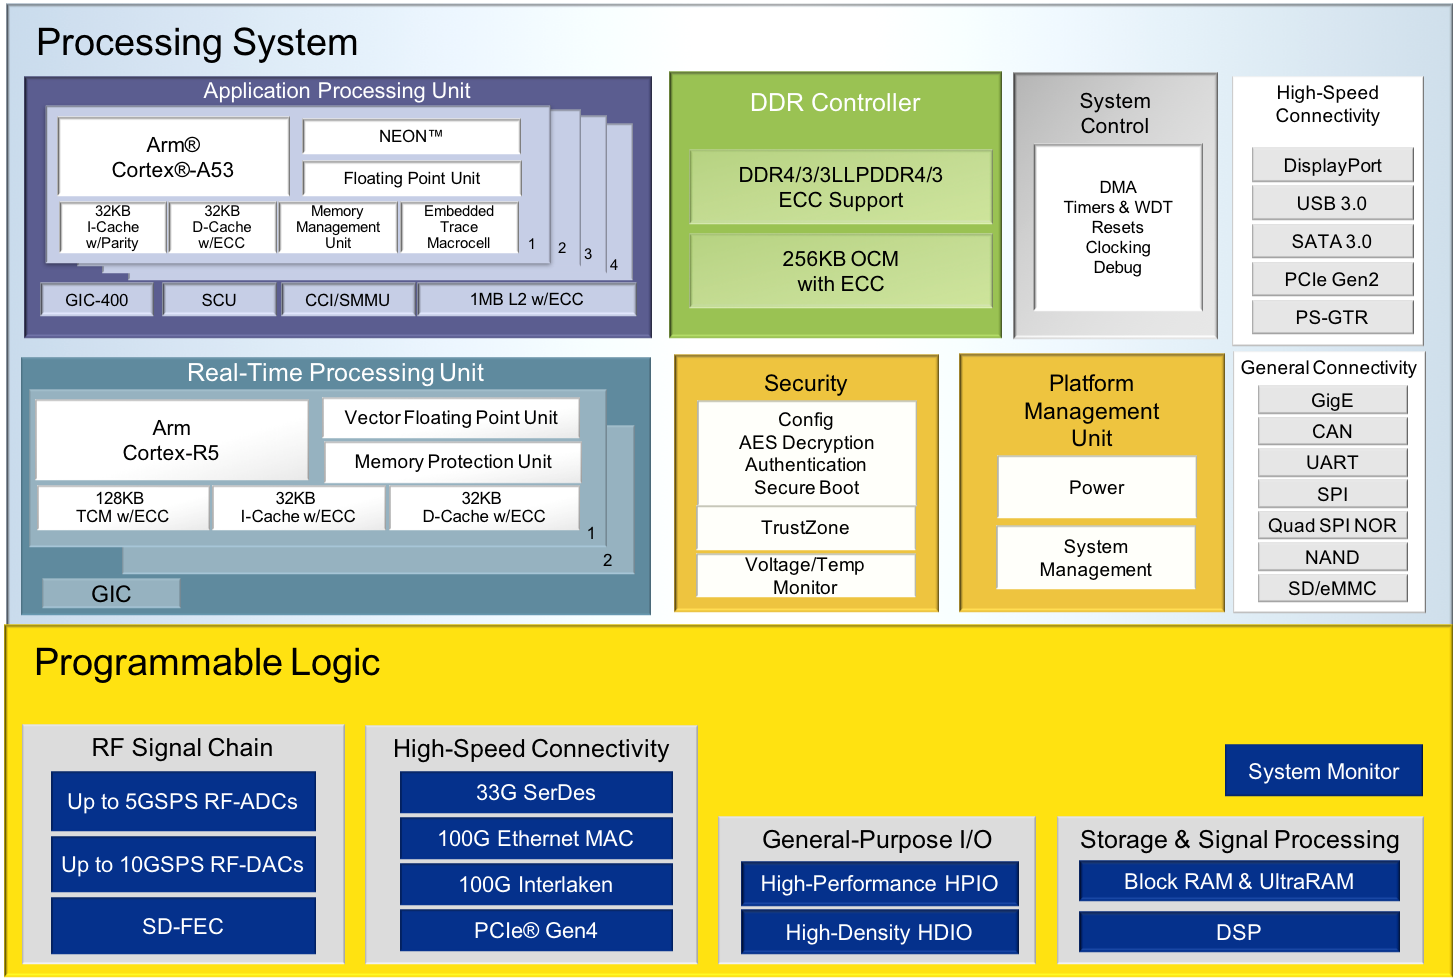
\includegraphics[width = \textwidth]{chap/04-work/img/rfsoc_blockdiagram}
	\caption{RFSoC block diagram}
	\label{fig:rfsoc}
\end{figure}

\section{Features}
\section{Evaluation Tool}